\documentclass{article}
\usepackage{tikz}
\usetikzlibrary{shapes,arrows}
\begin{document}

figure 1
  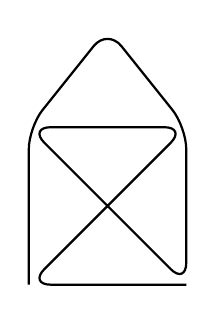
\begin{tikzpicture}
  \draw[thick,rounded corners=8pt] (0,0) -- (0,2) -- (1,3.25) 
   -- (2,2) -- (2,0) -- (0,2) -- (2,2) -- (0,0) -- (2,0);
  \end{tikzpicture}

figure 2
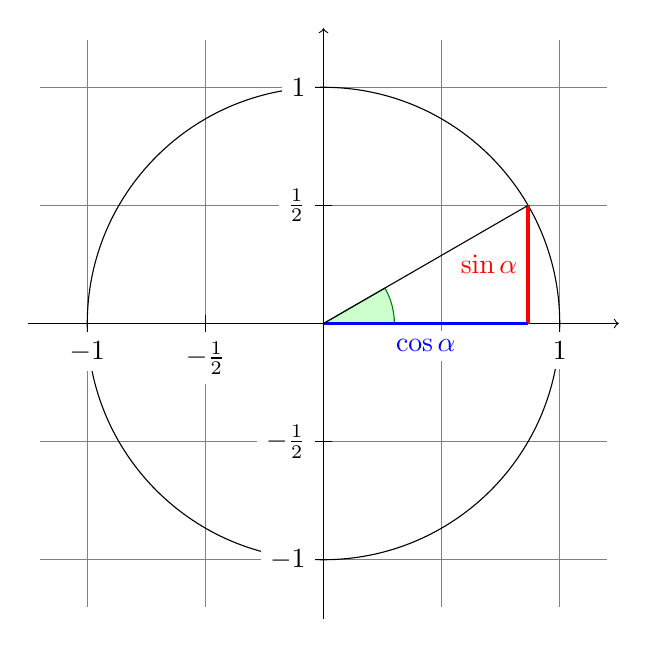
\begin{tikzpicture}[scale=3]
 \draw[step=.5cm, gray, very thin] (-1.2,-1.2) grid (1.2,1.2); 
 \filldraw[fill=green!20,draw=green!50!black] (0,0) -- (3mm,0mm) arc (0:30:3mm) -- cycle; 
 \draw[->] (-1.25,0) -- (1.25,0) coordinate (x axis);
 \draw[->] (0,-1.25) -- (0,1.25) coordinate (y axis);
 \draw (0,0) circle (1cm);
 \draw[very thick,red] (30:1cm) -- node[left,fill=white] {$\sin \alpha$} (30:1cm |- x axis);
 \draw[very thick,blue] (30:1cm |- x axis) -- node[below=2pt,fill=white] {$\cos \alpha$} (0,0);
 \draw (0,0) -- (30:1cm);
 \foreach \x/\xtext in {-1, -0.5/-\frac{1}{2}, 1} 
   \draw (\x cm,1pt) -- (\x cm,-1pt) node[anchor=north,fill=white] {$\xtext$};
 \foreach \y/\ytext in {-1, -0.5/-\frac{1}{2}, 0.5/\frac{1}{2}, 1} 
   \draw (1pt,\y cm) -- (-1pt,\y cm) node[anchor=east,fill=white] {$\ytext$};
 \end{tikzpicture}

figure 3
 \begin{tikzpicture}
    \draw (-1,0) to[bend left] (1,0);
    \draw (-1.2,.1) to[bend right] (1.2,.1);
    \draw[rotate=0] (0,0) ellipse (100pt and 50pt);
\end{tikzpicture}

figure 4
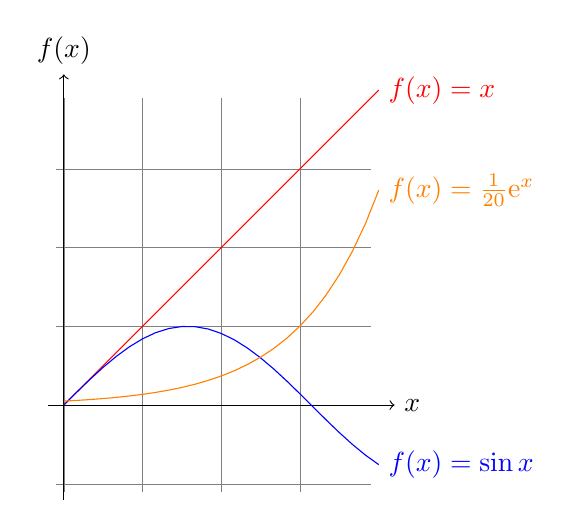
\begin{tikzpicture}[domain=0:4] 
    \draw[very thin,color=gray] (-0.1,-1.1) grid (3.9,3.9);
    \draw[->] (-0.2,0) -- (4.2,0) node[right] {$x$}; 
    \draw[->] (0,-1.2) -- (0,4.2) node[above] {$f(x)$};
    \draw[color=red]    plot (\x,\x)             node[right] {$f(x) =x$}; 
    \draw[color=blue]   plot (\x,{sin(\x r)})    node[right] {$f(x) = \sin x$}; 
    \draw[color=orange] plot (\x,{0.05*exp(\x)}) node[right] {$f(x) = \frac{1}{20} \mathrm e^x$};
  \end{tikzpicture}

\end{document}
